\chapter{Statistical Interpretation}
\section{Discovery Tests}
To test for the existence of signal in the observed dataset, the discovery tests discussed earlier are used to calculate p-values as a function of resonance mass. The results of these tests are shown in Figures \ref{fig:discov_hvtww} - \ref{fig:discov_rsg}. Across the different DY signals the largest excesses are $\sim 2.2\sigma$ at 600 GeV and $1.8\sigma$ at 2 TeV. The largest excesses for VBF signals are $< 2.5\sigma$ at for 1 TeV resonances. As these deviations do not constitute discoveries, upper limits on $\mu$ are calculated.
 \begin{figure}[h!]
  \centering
  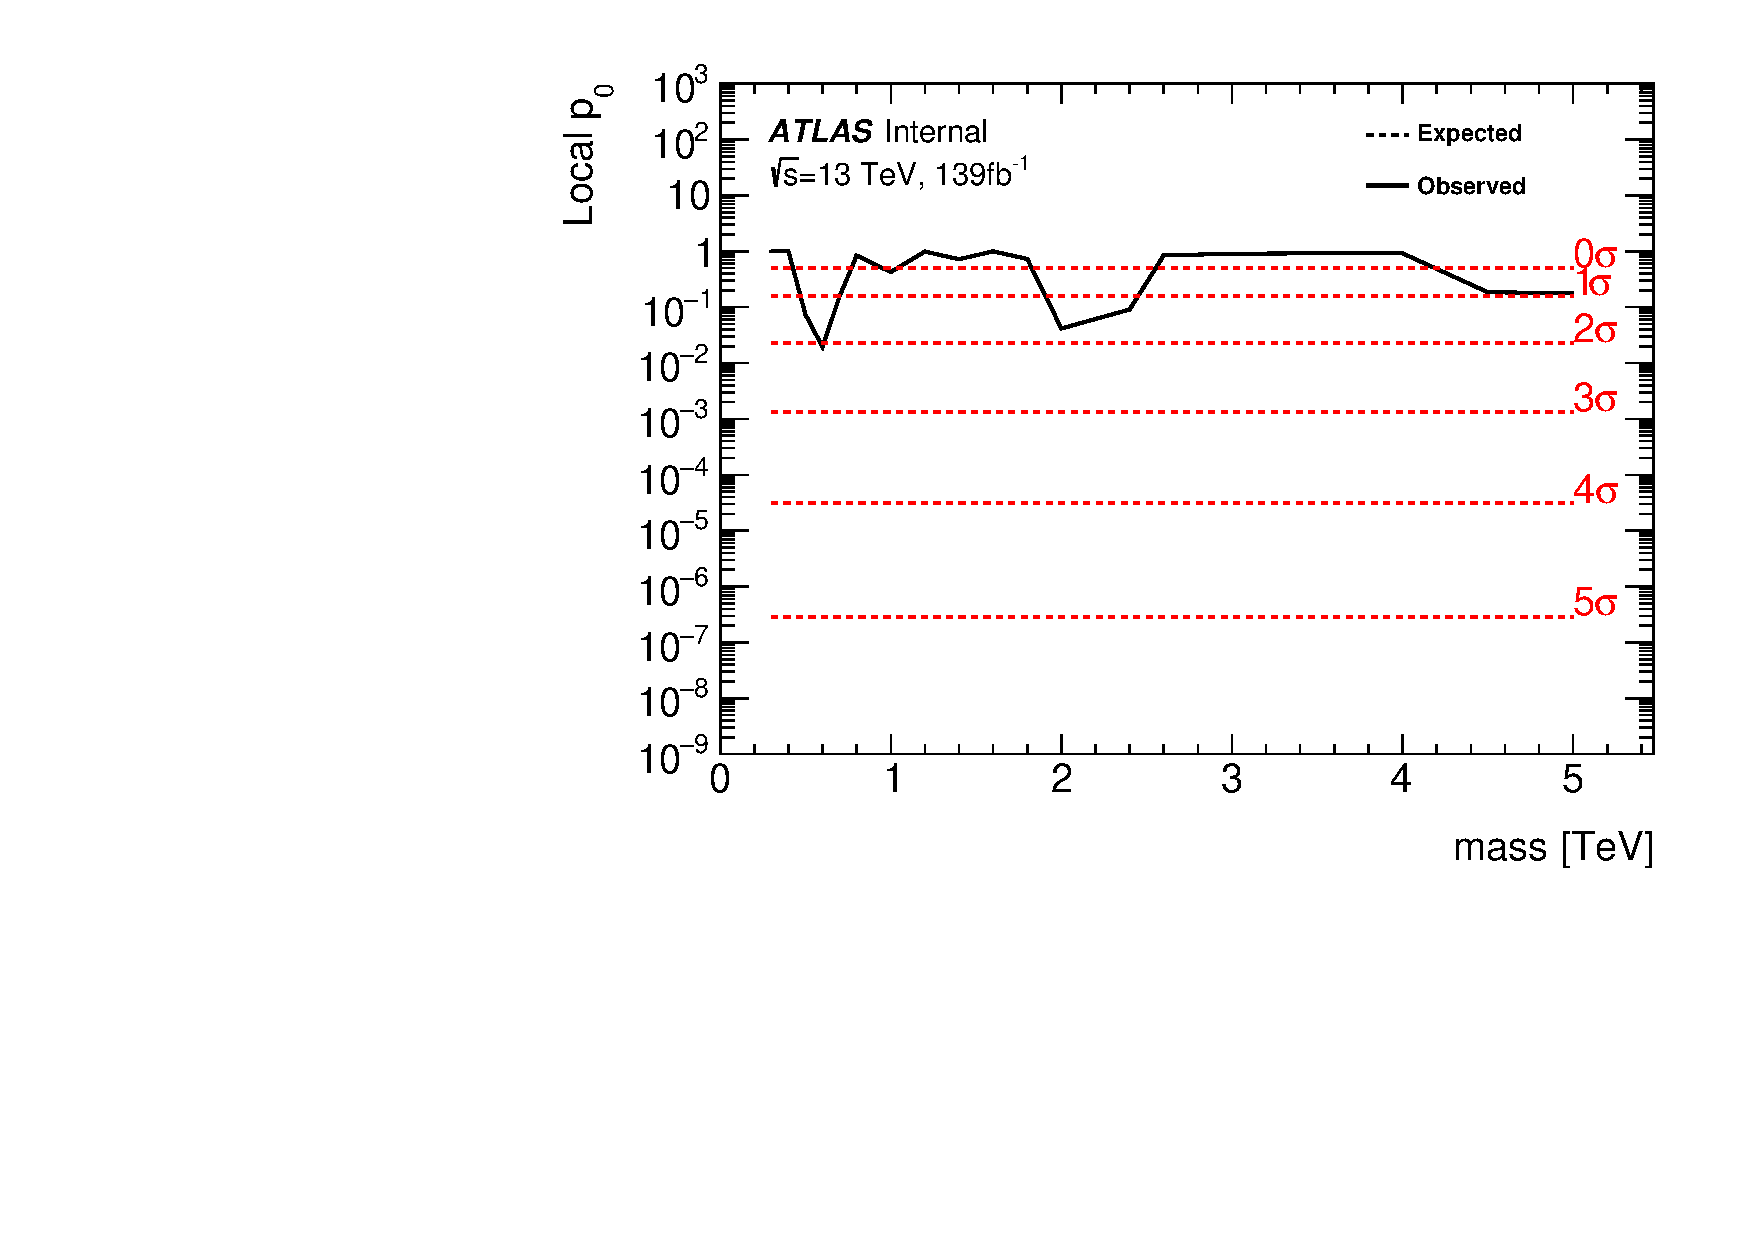
\includegraphics[width=\hsize]{figures/results/pvalues/hvtww_pvalue.pdf}
 \caption{These plots show the measured $p_{0}$ value as a function of resonance mass for HVT Z' DY production.} 
  \label{fig:discov_hvtww}
\end{figure} 
\FloatBarrier

\begin{figure}[h!]
  \centering
  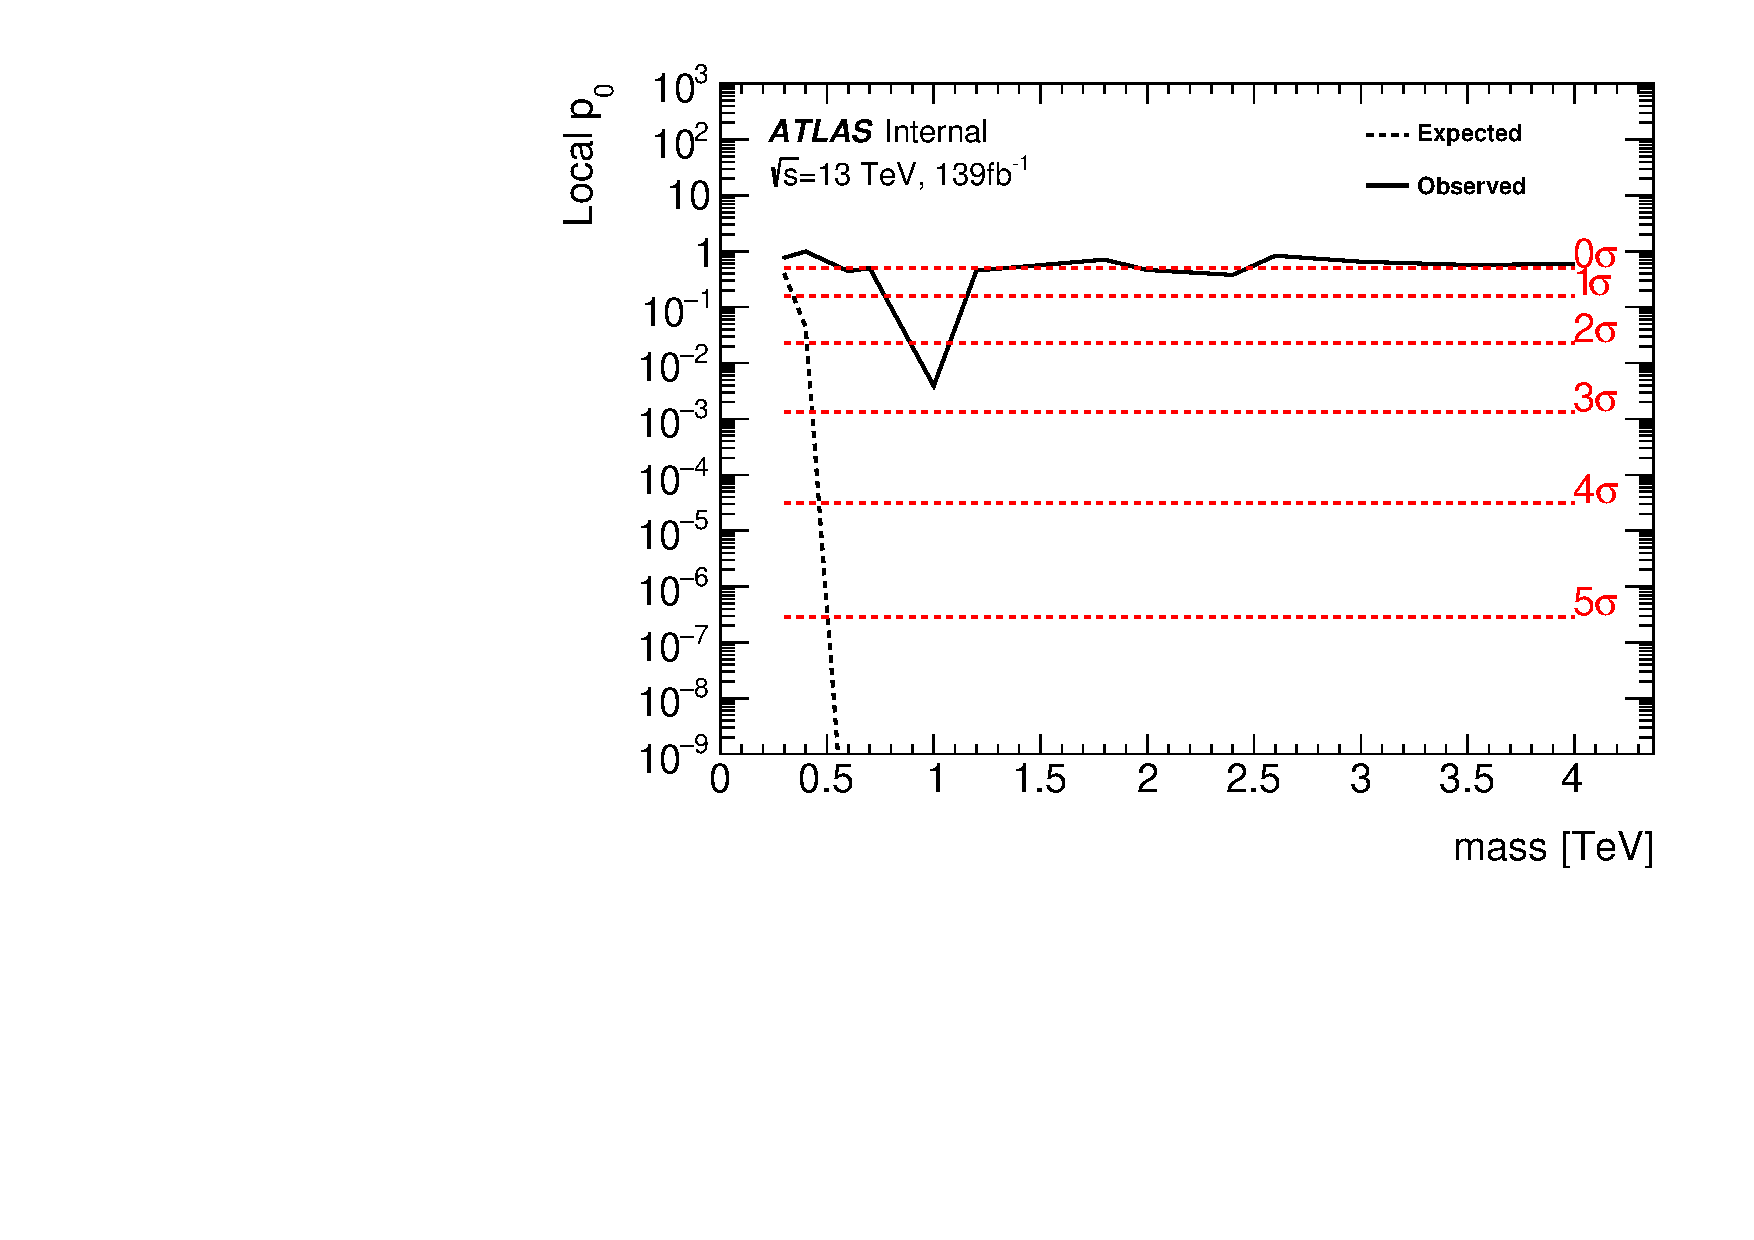
\includegraphics[width=\hsize]{figures/results/pvalues/hvtwwvbf_pvalue.pdf}
 \caption{These plots show the measured $p_{0}$ value as a function of resonance mass for HVT Z' VBF production.} 
  \label{fig:discov_hvtwwvbf}
\end{figure} 
\FloatBarrier


\begin{figure}[h!]
  \centering
  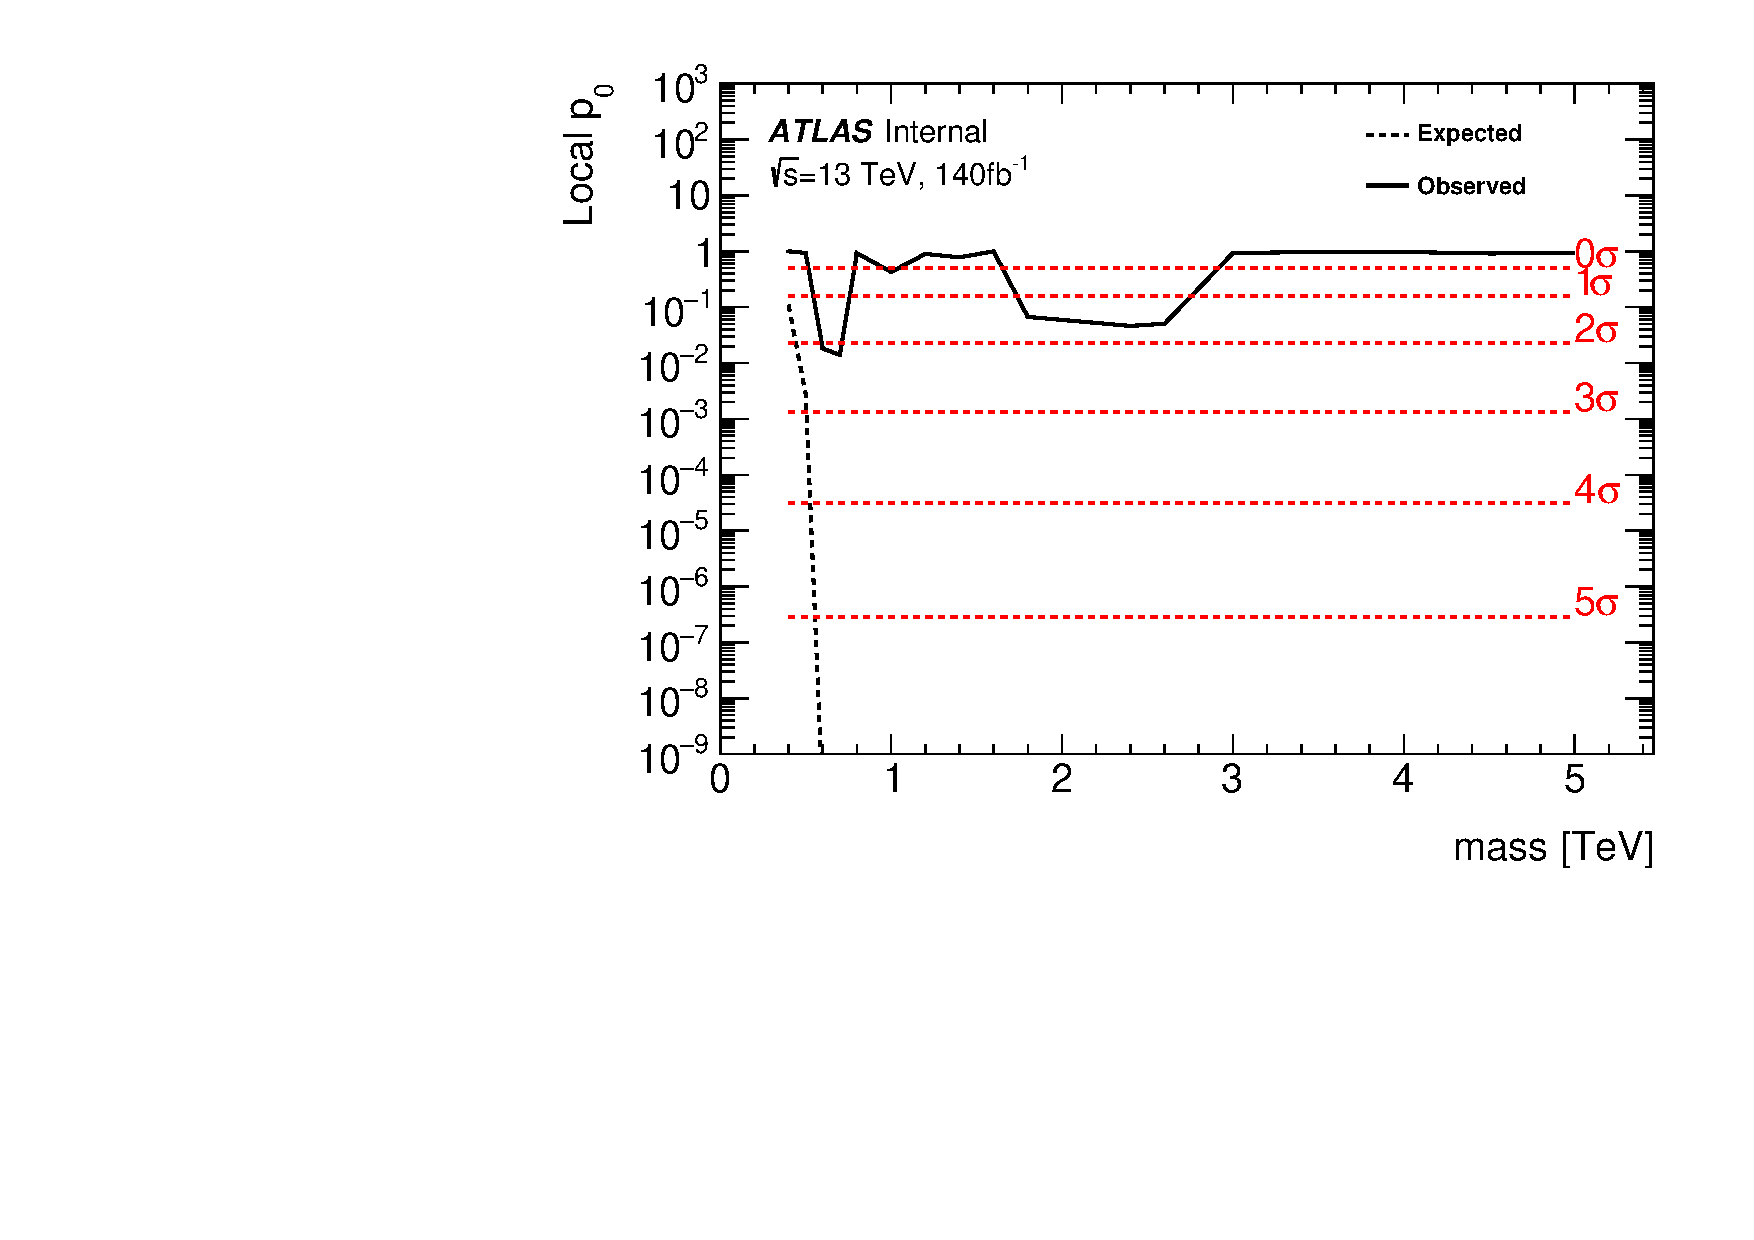
\includegraphics[width=\hsize]{figures/results/pvalues/hvtwz_pvalue.pdf}
 \caption{These plots show the measured $p_{0}$ value as a function of resonance mass for HVT W' DY production.} 
  \label{fig:discov_hvtwz}
\end{figure} 
\FloatBarrier

\begin{figure}[h!]
  \centering
  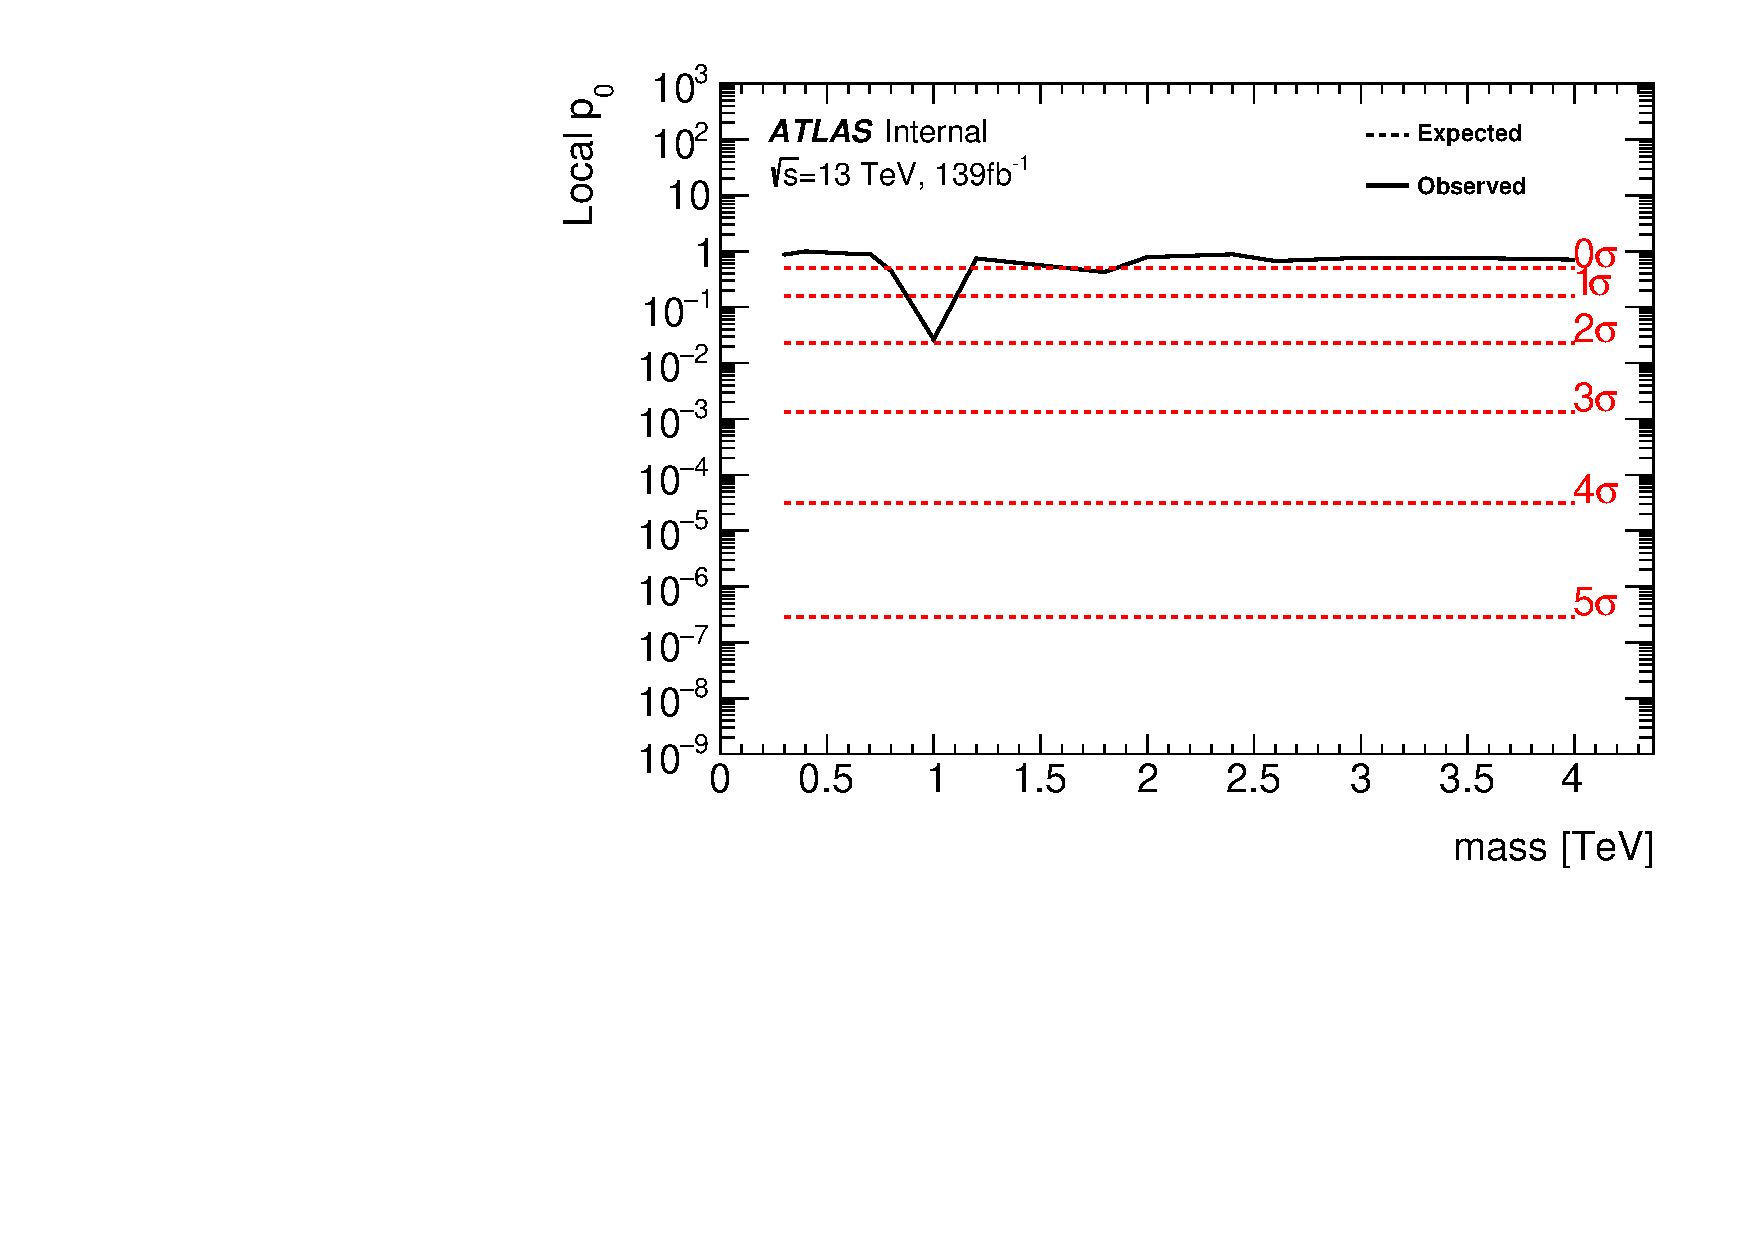
\includegraphics[width=\hsize]{figures/results/pvalues/hvtwzvbf_pvalue.pdf}
 \caption{These plots show the measured $p_{0}$ value as a function of resonance mass for HVT W' VBF production.} 
  \label{fig:discov_hvtwzvbf}
\end{figure} 
\FloatBarrier


\begin{figure}[h!]
  \centering
  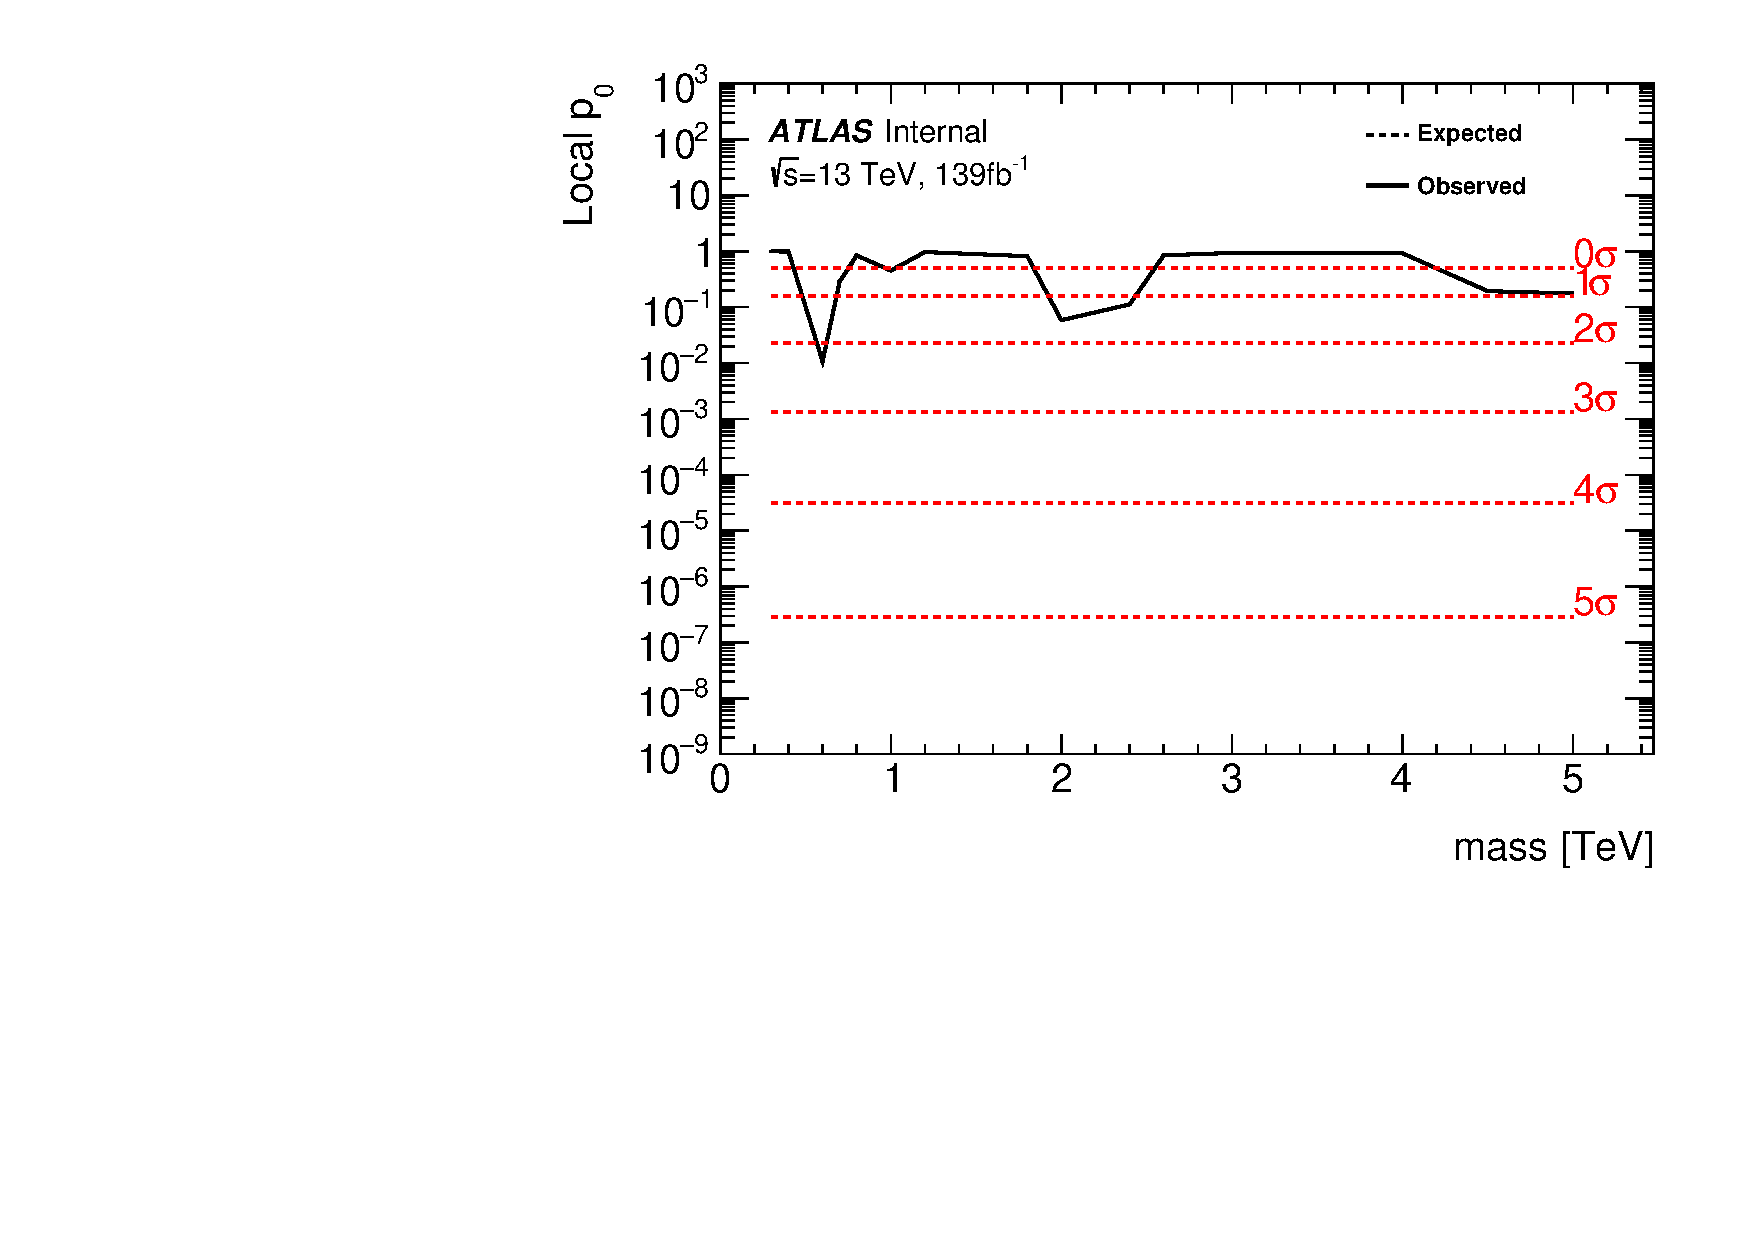
\includegraphics[width=\hsize]{figures/results/pvalues/rsg_pvalue.pdf}
 \caption{These plots show the measured $p_{0}$ value as a function of resonance mass for the RS Graviton DY production.} 
  \label{fig:discov_rsg}
\end{figure} 
\FloatBarrier
\section{Systematic Profiling and Correlations}
The ranked systematics and their fitted values are shown for the different analysis regions in Figure \ref{fig:hvtww_ranking} - \ref{fig:hvtwz_ranking}. Note that background normalizations for $W$+jets and $t\bar{t}$ are left free to float in the fit. This means the nominal normalization values are at one and the uncertainties are not plotted in the ranked plots. Overall, systematics are not pulled outside their uncertainties, especially for highly ranked nuisance parameters. 

The correlation between systematics are shown in Figures \ref{fig:hvtww_cor}. Correlations between background normalization are expected. The remaining systematic correlations are not very strong or unexpected.
\begin{figure}[h!]
  \centering
  \includegraphics[width=0.48\hsize]{figures/results/HVTWW/ranking_data/nov7_hvtww_2000gev/ranking.pdf}
    \includegraphics[width=0.48\hsize]{figures/results/HVTWWVBF/ranking_data/nov7_hvtwwvbf_1000gev/ranking.pdf}
 \caption{Ranked systematics and their fitted values for $WW$ DY (right) and VBF (left) selections.} 
  \label{fig:hvtww_ranking}
\end{figure} 
\FloatBarrier

\begin{figure}[h!]
  \centering
  \includegraphics[width=0.48\hsize]{figures/results/HVTWZ/ranking_data/nov7_hvtwz_1000gev/ranking.pdf}
    \includegraphics[width=0.48\hsize]{figures/results/HVTWZVBF/ranking_data/nov7_hvtwzvbf_1000gev/ranking.pdf}
 \caption{Ranked systematics and their fitted values for $WZ$ DY (right) and VBF (left) selections.} 
  \label{fig:hvtwz_ranking}
\end{figure} 
\FloatBarrier

\begin{figure}[h!]
  \centering
  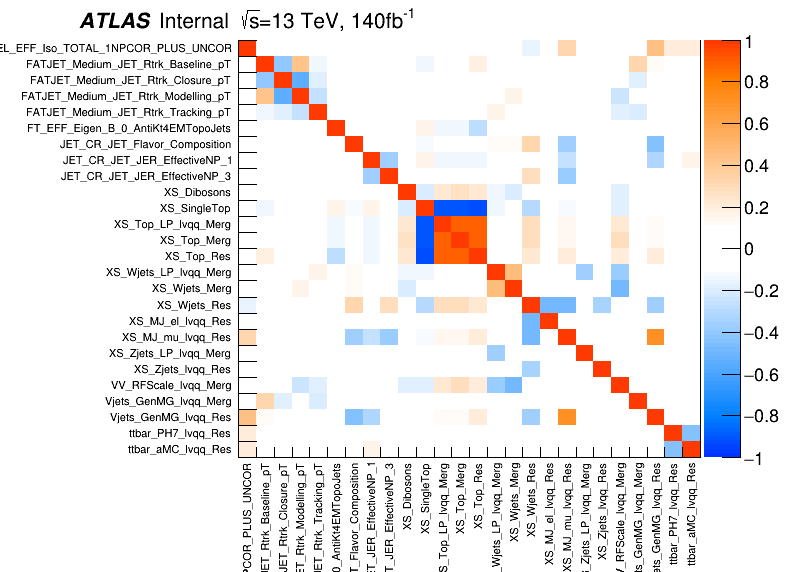
\includegraphics[width=0.48\hsize]{figures/Results/HVTWW/HVTWW_combined_1nov8_maybeFloatRelevantUncorrXSSingleBinPrunSyst/Plots/CorrMatrix/corr_doAsimov0_doCondtional1_mu0_HighCorr.png}
   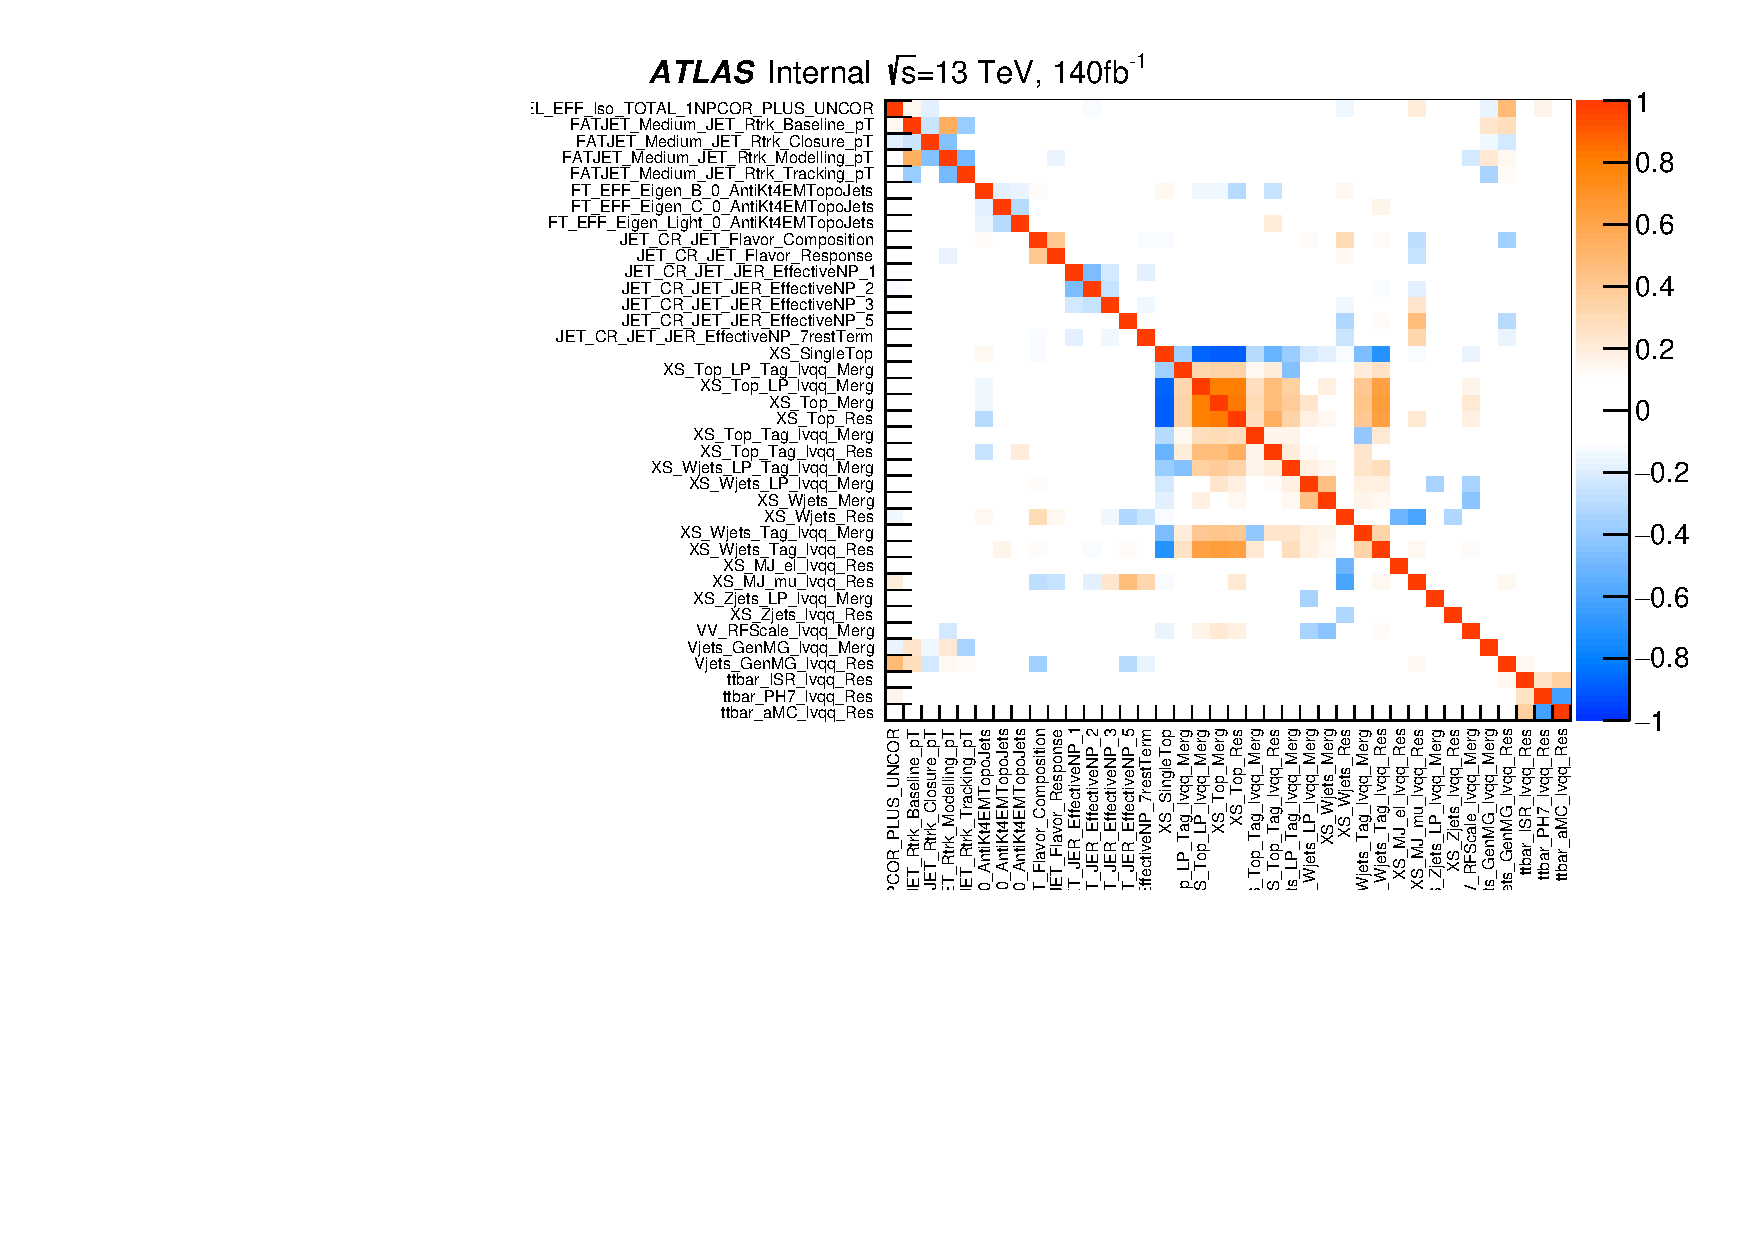
\includegraphics[width=0.48\hsize]{figures/Results/HVTWWVBF/HVTWWVBF_combined_1nov8_maybeFloatRelevantUncorrXSSingleBinPrunSyst/Plots/CorrMatrix/corr_doAsimov0_doCondtional1_mu0_HighCorr.pdf}
 \caption{Correlations between systematics for $WW$ DY (right) and VBF (left) selections.} 
  \label{fig:hvtwz_ranking}
\end{figure} 
\FloatBarrier
\section{Expected and Measured Yields}
The yield tables for the four analysis regions are shown in Tables \ref{tbl:hvtww_yields} - \ref{tbl:hvwzvbf_yields}. The fitted background normalizations are shown in Tables \ref{tbl:hvtww_xs_fit}-\ref{tbl:hvtwzvbf_xs_fit}

% Postfit L1 GGF WCR  
\begin{table}
\begin{tabular}{|l|c|c|c|}
\hline
	  &	 HP WCR &	 LP WCR &	Resolved WCR \\\hline 
	%HVT Z' &	3.91 $\pm$ 9.88 &	7.05 $\pm$ 17.83 &	0.42 $\pm$ 1.06 \\\hline 
	Electron Multi-jet &	- &	- &	16507.83 $\pm$ 2314.87 \\\hline 
	Muon Multi-jet &	- &	- &	19977.12 $\pm$ 2816.06 \\\hline 
	Diboson &	1833.41 $\pm$ 177.78 &	3323.93 $\pm$ 320.92 &	9147.67 $\pm$ 961.63 \\\hline 
	Single-top &	2160.62 $\pm$ 402.34 &	3551.09 $\pm$ 660.00 &	20058.36 $\pm$ 3817.26 \\\hline 
	$t\bar{t}$ &	15518.86 $\pm$ 338.22 &	24069.54 $\pm$ 453.15 &	138866.23 $\pm$ 1989.71 \\\hline 
	$W$+jets &	40141.57 $\pm$ 357.79 &	88113.06 $\pm$ 487.87 &	673200.38 $\pm$ 4120.53 \\\hline 
	$Z$+jets &	778.83 $\pm$ 78.93 &	1765.54 $\pm$ 179.10 &	16570.50 $\pm$ 1672.71 \\\hline 
	Total &	60433.29 $\pm$ 664.92 &	120823.16 $\pm$ 1006.99 &	894328.12 $\pm$ 7247.12 \\\hline 
	Data &	60264.00 &	120852.00 &	895362.00 \\\hline 
\end{tabular}


% Postfit L1 GGF TCR 
 
\begin{tabular}{|l|c|c|c|}
\hline
	  &	 HP  TCR &	 LP  TCR &	Resolved TCR \\\hline 
	%HVT Z' &	1.27 $\pm$ 3.20 &	0.60 $\pm$ 1.50 &	0.12 $\pm$ 0.30 \\\hline 
	Electron Multi-jet &	- &	- &	- \\\hline 
	Muon Multi-jet &	- &	- &	- \\\hline 
	Diboson &	421.11 $\pm$ 37.98 &	550.44 $\pm$ 53.10 &	996.87 $\pm$ 119.63 \\\hline 
	Single-top &	4691.44 $\pm$ 846.11 &	3466.26 $\pm$ 631.03 &	16848.71 $\pm$ 3258.26 \\\hline 
	$t\bar{t}$ &	38945.18 $\pm$ 848.77 &	33836.95 $\pm$ 637.04 &	224226.14 $\pm$ 3212.76 \\\hline 
	$W$+jets &	2258.34 $\pm$ 20.13 &	6564.78 $\pm$ 36.35 &	23466.41 $\pm$ 143.63 \\\hline 
	$Z$+jets &	66.35 $\pm$ 6.72 &	213.26 $\pm$ 21.63 &	846.66 $\pm$ 85.47 \\\hline 
	Total &	46382.43 $\pm$ 1199.25 &	44631.70 $\pm$ 899.23 &	266384.78 $\pm$ 4580.43 \\\hline 
	Data &	46354.00 &	44629.00 &	266443.00 \\\hline 
\end{tabular}

% Postfit L1 GGF SR  
\begin{tabular}{|l|c|c|c|}
\hline
	  &	 WW SR &	 LP SR &	Resolved 1-lepton SR \\\hline 
	%HVT Z' &	21.59 $\pm$ 54.38 &	10.39 $\pm$ 25.86 &	4.22 $\pm$ 10.58 \\\hline 
	Electron Multi-jet &	- &	- &	10788.40 $\pm$ 1512.85 \\\hline 
	Muon Multi-jet &	- &	- &	15759.50 $\pm$ 2221.53 \\\hline 
	Diboson &	4990.30 $\pm$ 376.50 &	3901.07 $\pm$ 313.22 &	16971.29 $\pm$ 1523.77 \\\hline 
	Single-top &	3117.71 $\pm$ 565.07 &	2176.46 $\pm$ 400.52 &	20422.85 $\pm$ 3731.94 \\\hline 
	$t\bar{t}$ &	13785.77 $\pm$ 302.14 &	11005.12 $\pm$ 207.41 &	126965.25 $\pm$ 1819.66 \\\hline 
	$W$+jets &	24718.56 $\pm$ 223.72 &	60080.66 $\pm$ 333.12 &	444133.56 $\pm$ 2719.02 \\\hline 
	$Z$+jets &	478.18 $\pm$ 48.46 &	1226.69 $\pm$ 124.44 &	11686.32 $\pm$ 1179.69 \\\hline 
	Total &	47090.52 $\pm$ 777.65 &	78389.98 $\pm$ 654.22 &	646727.19 $\pm$ 5963.98 \\\hline 
	Data &	47330.00 &	78380.00 &	645610.00 \\\hline 
\end{tabular}
\caption{Expected and Measured for DY $WW$ $W$+jets, $t\bar{t}$ control regions and signal regions.}
\label{tbl:hvtww_yields_tcr}
\end{table}

\begin{table}
% Postfit L1 GGF WCR Untag 
\begin{tabular}{|l|c|c|c|}
\hline
	  &	 HP  Untagged WCR &	 LP Untagged WCR &	Resolved Untagged WCR \\\hline 
	%HVT W' &	2.31 $\pm$ 5.75 &	3.63 $\pm$ 9.18 &	0.73 $\pm$ 1.83 \\\hline 
	Electron Multi-jet &	- &	- &	15080.03 $\pm$ 2277.99 \\\hline 
	Muon Multi-jet &	- &	- &	27347.10 $\pm$ 2950.07 \\\hline 
	Diboson &	1508.48 $\pm$ 154.20 &	2758.24 $\pm$ 284.50 &	9038.55 $\pm$ 728.69 \\\hline 
	Single-top &	1756.59 $\pm$ 306.69 &	2913.18 $\pm$ 515.93 &	20511.74 $\pm$ 3523.47 \\\hline 
	$t\bar{t}$ &	13134.00 $\pm$ 238.30 &	21815.37 $\pm$ 334.98 &	140157.77 $\pm$ 2636.96 \\\hline 
	$W$+jets &	40654.84 $\pm$ 333.65 &	87657.76 $\pm$ 501.96 &	665909.12 $\pm$ 4420.62 \\\hline 
	$Z$+jets &	768.72 $\pm$ 77.97 &	1759.87 $\pm$ 178.96 &	16512.46 $\pm$ 1673.23 \\\hline 
	Total &	57822.63 $\pm$ 540.40 &	116904.42 $\pm$ 862.16 &	894556.75 $\pm$ 7492.20 \\\hline 
	Data &	57699.00 &	117306.00 &	895362.00 \\\hline 
\end{tabular}

% Postfit L1 GGF WCR Tag 

\begin{tabular}{|l|c|c|c|}
\hline
	  &	 HP Tagged WCR &	 LP Tagged WCR &	Resolved Tagged WCR \\\hline 
%	HVT W' &	0.45 $\pm$ 1.12 &	0.86 $\pm$ 2.18 &	0.18 $\pm$ 0.44 \\\hline 
	Electron Multi-jet &	- &	- &	384.58 $\pm$ 57.11 \\\hline 
	Muon Multi-jet &	- &	- &	602.93 $\pm$ 190.12 \\\hline 
	Diboson &	30.22 $\pm$ 4.69 &	48.95 $\pm$ 7.16 &	264.64 $\pm$ 28.24 \\\hline 
	Single-top &	308.44 $\pm$ 56.19 &	371.59 $\pm$ 69.43 &	5752.39 $\pm$ 1029.97 \\\hline 
	$t\bar{t}$ &	1683.82 $\pm$ 48.73 &	2041.48 $\pm$ 70.00 &	58431.49 $\pm$ 614.30 \\\hline 
	$W$+jets &	583.55 $\pm$ 75.37 &	1109.45 $\pm$ 85.78 &	11891.68 $\pm$ 903.01 \\\hline 
	$Z$+jets &	13.19 $\pm$ 1.34 &	23.06 $\pm$ 2.34 &	324.74 $\pm$ 32.85 \\\hline 
	Total &	2619.22 $\pm$ 106.00 &	3594.53 $\pm$ 130.90 &	77652.45 $\pm$ 1514.89 \\\hline 
	Data &	2565.00 &	3546.00 &	77973.00 \\\hline 
\end{tabular}

% Postfit L1 GGF TCR Untag 
\begin{tabular}{|l|c|c|c|}
\hline
	  &	 HP Untagged TCR &	 LP Untagged TCR &	Resolved Untagged TCR \\\hline 
%	HVT W' &	0.75 $\pm$ 1.87 &	0.33 $\pm$ 0.81 &	0.10 $\pm$ 0.25 \\\hline 
	Electron Multi-jet &	- &	- &	- \\\hline 
	Muon Multi-jet &	- &	- &	- \\\hline 
	Diboson &	289.45 $\pm$ 28.45 &	346.78 $\pm$ 35.85 &	650.85 $\pm$ 65.56 \\\hline 
	Single-top &	3107.99 $\pm$ 538.03 &	2250.64 $\pm$ 385.41 &	9606.87 $\pm$ 1698.22 \\\hline 
	$t\bar{t}$ &	30992.40 $\pm$ 562.33 &	26954.21 $\pm$ 413.89 &	91893.59 $\pm$ 1728.91 \\\hline 
	$W$+jets &	2236.29 $\pm$ 18.35 &	4874.03 $\pm$ 27.91 &	16122.97 $\pm$ 107.03 \\\hline 
	$Z$+jets &	71.54 $\pm$ 7.26 &	155.50 $\pm$ 15.81 &	577.71 $\pm$ 58.54 \\\hline 
	Total &	36697.66 $\pm$ 779.03 &	34581.16 $\pm$ 567.59 &	118851.98 $\pm$ 2427.40 \\\hline 
	Data &	36677.00 &	34573.00 &	118928.00 \\\hline 
\end{tabular}

% Postfit L1 GGF TCR Tag 
\begin{tabular}{|l|c|c|c|}
\hline
	  &	 HP Tagged TCR &	 LP Tagged TCR &	Resolved Tagged TCR \\\hline 
%	HVT W' &	0.12 $\pm$ 0.31 &	0.05 $\pm$ 0.13 &	0.02 $\pm$ 0.04 \\\hline 
	Electron Multi-jet &	- &	- &	- \\\hline 
	Muon Multi-jet &	- &	- &	- \\\hline 
	Diboson &	9.72 $\pm$ 1.13 &	8.75 $\pm$ 1.16 &	34.06 $\pm$ 4.98 \\\hline 
	Single-top &	105.87 $\pm$ 20.65 &	119.66 $\pm$ 22.68 &	656.89 $\pm$ 132.96 \\\hline 
	$t\bar{t}$ &	1904.75 $\pm$ 50.61 &	1483.86 $\pm$ 47.05 &	17965.33 $\pm$ 188.87 \\\hline 
	$W$+jets &	32.36 $\pm$ 4.28 &	85.74 $\pm$ 6.96 &	489.01 $\pm$ 37.13 \\\hline 
	$Z$+jets &	1.27 $\pm$ 0.13 &	1.93 $\pm$ 0.20 &	19.14 $\pm$ 1.94 \\\hline 
	Total &	2053.98 $\pm$ 54.84 &	1699.93 $\pm$ 52.70 &	19164.43 $\pm$ 234.01 \\\hline 
	Data &	2047.00 &	1708.00 &	19143.00 \\\hline 
\end{tabular}


\caption{Expected and Measured for DY $WZ$ $W$+jets, $t\bar{t}$ tag and untag control regions.}
\label{tbl:hvtwz_yields_cr}
\end{table}

\begin{table}
% Postfit L1 GGF SR Untag 
\begin{tabular}{|l|c|c|c|}
\hline
	  &	 HP Untagged SR &	 LP Untagged SR &	Resolved Untagged SR \\\hline 
%	HVT W' &	13.08 $\pm$ 32.55 &	5.65 $\pm$ 14.09 &	3.73 $\pm$ 9.29 \\\hline 
	Electron Multi-jet &	- &	- &	7782.17 $\pm$ 1175.56 \\\hline 
	Muon Multi-jet &	- &	- &	17004.81 $\pm$ 1834.40 \\\hline 
	Diboson &	3041.17 $\pm$ 273.77 &	2266.35 $\pm$ 212.79 &	14724.12 $\pm$ 1224.31 \\\hline 
	Single-top &	2123.28 $\pm$ 373.83 &	1379.35 $\pm$ 240.92 &	18336.88 $\pm$ 3082.47 \\\hline 
	$t\bar{t}$ &	11678.86 $\pm$ 213.63 &	8906.34 $\pm$ 136.88 &	112669.24 $\pm$ 2122.46 \\\hline 
	$W$+jets &	22741.32 $\pm$ 191.47 &	41726.76 $\pm$ 240.56 &	342934.00 $\pm$ 2280.21 \\\hline 
	$Z$+jets &	442.03 $\pm$ 44.84 &	849.79 $\pm$ 86.42 &	9271.83 $\pm$ 939.52 \\\hline 
	Total &	40026.65 $\pm$ 546.81 &	55128.59 $\pm$ 432.90 &	522723.03 $\pm$ 5131.71 \\\hline 
	Data &	40193.00 &	54735.00 &	521813.00 \\\hline 
\end{tabular}

% Postfit L1 GGF SR Tag 
\begin{tabular}{|l|c|c|c|}
\hline
	  &	 HP Tagged SR &	 LP Tagged SR &	Resolved Tagged SR \\\hline 
%	HVT W' &	2.20 $\pm$ 5.48 &	1.01 $\pm$ 2.53 &	1.00 $\pm$ 2.48 \\\hline 
	Electron Multi-jet &	- &	- &	199.22 $\pm$ 29.58 \\\hline 
	Muon Multi-jet &	- &	- &	393.43 $\pm$ 124.06 \\\hline 
	Diboson &	102.58 $\pm$ 11.59 &	65.44 $\pm$ 8.05 &	624.07 $\pm$ 58.10 \\\hline 
	Single-top &	178.21 $\pm$ 33.62 &	155.53 $\pm$ 28.95 &	3470.39 $\pm$ 617.48 \\\hline 
	$t\bar{t}$ &	1017.93 $\pm$ 31.95 &	706.76 $\pm$ 26.20 &	38189.30 $\pm$ 401.91 \\\hline 
	$W$+jets &	325.58 $\pm$ 41.62 &	575.36 $\pm$ 43.29 &	6161.96 $\pm$ 467.71 \\\hline 
	$Z$+jets &	7.81 $\pm$ 0.80 &	11.62 $\pm$ 1.19 &	183.36 $\pm$ 18.55 \\\hline 
	Total &	1632.11 $\pm$ 63.39 &	1514.70 $\pm$ 58.86 &	49221.74 $\pm$ 884.06 \\\hline 
	Data &	1699.00 &	1559.00 &	48919.00 \\\hline 
\end{tabular}
\caption{Expected and Measured for DY $WZ$ $W$+jets, $t\bar{t}$ tag and untag signal regions.}
\label{tbl:hvtwz_yields_tcr}
\end{table}

\begin{table}
% Postfit L1 VBF WCR 
\begin{tabular}{|l|c|c|c|}
\hline
	  &	 HP WCR &	 LP WCR &	Resolved WCR \\\hline 
	%HVT VBF Z' &	6.05 $\pm$ 2.78 &	12.08 $\pm$ 8.55 &	1.62 $\pm$ 0.72 \\\hline 
	Electron Multi-jet &	- &	- &	898.48 $\pm$ 137.82 \\\hline 
	Muon Multi-jet &	- &	- &	601.46 $\pm$ 182.74 \\\hline 
	Diboson &	107.45 $\pm$ 45.20 &	166.87 $\pm$ 68.11 &	292.10 $\pm$ 235.29 \\\hline 
	Single-top &	78.19 $\pm$ 18.22 &	132.71 $\pm$ 31.93 &	879.82 $\pm$ 216.89 \\\hline 
	$t\bar{t}$ &	400.71 $\pm$ 28.35 &	569.70 $\pm$ 48.88 &	5067.51 $\pm$ 155.69 \\\hline 
	$W$+jets &	864.49 $\pm$ 63.44 &	1940.80 $\pm$ 89.41 &	18563.70 $\pm$ 408.99 \\\hline 
	$Z$+jets &	19.51 $\pm$ 2.00 &	46.63 $\pm$ 4.77 &	795.20 $\pm$ 80.89 \\\hline 
	Total &	1470.35 $\pm$ 84.89 &	2856.71 $\pm$ 126.74 &	27098.28 $\pm$ 594.01 \\\hline 
	Data &	1495.00 &	2898.00 &	27120.00 \\\hline 
\end{tabular}

% Postfit L1 VBF TCR 
\begin{tabular}{|l|c|c|c|}
\hline
	  &	 HP TCR &	 LP TCR &	Resolved TCR \\\hline 
%	HVT VBF Z' &	1.84 $\pm$ 0.72 &	1.15 $\pm$ 0.57 &	0.62 $\pm$ 0.28 \\\hline 
	Electron Multi-jet &	- &	- &	- \\\hline 
	Muon Multi-jet &	- &	- &	- \\\hline 
	Diboson &	14.95 $\pm$ 6.61 &	27.57 $\pm$ 14.12 &	24.33 $\pm$ 20.32 \\\hline 
	Single-top &	68.31 $\pm$ 16.17 &	58.93 $\pm$ 13.56 &	278.60 $\pm$ 73.04 \\\hline 
	$t\bar{t}$ &	496.60 $\pm$ 31.72 &	401.23 $\pm$ 32.13 &	3834.49 $\pm$ 104.60 \\\hline 
	$W$+jets &	50.68 $\pm$ 4.19 &	144.02 $\pm$ 7.86 &	450.01 $\pm$ 11.87 \\\hline 
	$Z$+jets &	1.32 $\pm$ 0.14 &	5.35 $\pm$ 0.55 &	29.96 $\pm$ 3.07 \\\hline 
	Total &	631.87 $\pm$ 36.45 &	637.10 $\pm$ 38.44 &	4617.39 $\pm$ 129.77 \\\hline 
	Data &	636.00 &	634.00 &	4615.00 \\\hline 
\end{tabular}

% Postfit L1 VBF SR 
\begin{tabular}{|l|c|c|c|}
\hline
	  &	 HP SR &	 LP SR &	Resolved SR \\\hline 
%	HVT VBF Z' &	38.90 $\pm$ 15.11 &	19.28 $\pm$ 9.38 &	20.33 $\pm$ 8.96 \\\hline 
	Electron Multi-jet &	- &	- &	596.34 $\pm$ 91.52 \\\hline 
	Muon Multi-jet &	- &	- &	481.01 $\pm$ 144.48 \\\hline 
	Diboson &	148.84 $\pm$ 48.64 &	181.42 $\pm$ 67.30 &	395.52 $\pm$ 318.06 \\\hline 
	Single-top &	79.49 $\pm$ 19.80 &	56.82 $\pm$ 14.89 &	782.07 $\pm$ 190.79 \\\hline 
	$t\bar{t}$ &	338.42 $\pm$ 24.14 &	236.80 $\pm$ 20.88 &	4261.70 $\pm$ 138.98 \\\hline 
	$W$+jets &	501.13 $\pm$ 39.36 &	1347.76 $\pm$ 64.50 &	11445.73 $\pm$ 291.49 \\\hline 
	$Z$+jets &	9.25 $\pm$ 0.95 &	28.77 $\pm$ 2.95 &	567.66 $\pm$ 57.94 \\\hline 
	Total &	1077.13 $\pm$ 69.93 &	1851.57 $\pm$ 96.73 &	18530.03 $\pm$ 523.88 \\\hline 
	Data &	1096.00 &	1846.00 &	18530.00 \\\hline 
\end{tabular}
\caption{Expected and Measured for VBF $WW$ $W$+jets, $t\bar{t}$ control regions and signal regions.}
\label{tbl:hvtwvbf_yields_tcr}
\end{table}

\begin{table}

% Postfit L1 VBF WCR  
\begin{tabular}{|l|c|c|c|}
\hline
	  &	 HP WCR &	 LP WCR &	Resolved WCR \\\hline 
%	HVT VBF W' &	3.57 $\pm$ 2.00 &	5.91 $\pm$ 4.43 &	1.90 $\pm$ 1.07 \\\hline 
	Electron Multi-jet &	- &	- &	870.00 $\pm$ 132.75 \\\hline 
	Muon Multi-jet &	- &	- &	618.45 $\pm$ 196.90 \\\hline 
	Diboson &	92.92 $\pm$ 41.77 &	145.90 $\pm$ 64.26 &	228.62 $\pm$ 114.62 \\\hline 
	Single-top &	71.13 $\pm$ 16.29 &	118.82 $\pm$ 27.98 &	1209.87 $\pm$ 281.64 \\\hline 
	$t\bar{t}$ &	427.80 $\pm$ 29.72 &	509.19 $\pm$ 46.57 &	6860.87 $\pm$ 254.83 \\\hline 
	$W$+jets &	871.68 $\pm$ 64.22 &	2020.67 $\pm$ 93.54 &	19088.50 $\pm$ 442.10 \\\hline 
	$Z$+jets &	19.58 $\pm$ 2.01 &	47.39 $\pm$ 4.85 &	800.19 $\pm$ 82.02 \\\hline 
	Total &	1483.11 $\pm$ 83.79 &	2841.97 $\pm$ 125.92 &	29676.50 $\pm$ 644.96 \\\hline 
	Data &	1495.00 &	2898.00 &	29755.00 \\\hline 
\end{tabular}

% Postfit L1 VBF TCR  
\begin{tabular}{|l|c|c|c|}
\hline
	  &	 HP TCR &	 LP TCR &	Resolved TCR \\\hline 
	%HVT VBF W' &	1.42 $\pm$ 0.75 &	0.79 $\pm$ 0.47 &	0.53 $\pm$ 0.30 \\\hline 
	Electron Multi-jet &	- &	- &	- \\\hline 
	Muon Multi-jet &	- &	- &	- \\\hline 
	Diboson &	10.12 $\pm$ 4.51 &	12.73 $\pm$ 6.55 &	14.23 $\pm$ 7.49 \\\hline 
	Single-top &	51.57 $\pm$ 12.31 &	35.07 $\pm$ 8.17 &	169.21 $\pm$ 44.54 \\\hline 
	$t\bar{t}$ &	470.06 $\pm$ 28.97 &	298.99 $\pm$ 25.28 &	2414.75 $\pm$ 75.42 \\\hline 
	$W$+jets &	49.64 $\pm$ 4.17 &	109.69 $\pm$ 6.16 &	378.22 $\pm$ 12.05 \\\hline 
	$Z$+jets &	1.28 $\pm$ 0.13 &	4.81 $\pm$ 0.50 &	17.62 $\pm$ 1.83 \\\hline 
	Total &	582.67 $\pm$ 32.07 &	461.30 $\pm$ 28.05 &	2994.03 $\pm$ 88.75 \\\hline 
	Data &	584.00 &	459.00 &	3001.00 \\\hline 
\end{tabular}

% Postfit L1 VBF SR  
\begin{tabular}{|l|c|c|c|}
\hline
	  &	 HP SR &	 LP SR &	Resolved SR \\\hline 
	%HVT VBF W' &	27.77 $\pm$ 14.54 &	12.44 $\pm$ 7.29 &	17.01 $\pm$ 9.36 \\\hline 
	Electron Multi-jet &	- &	- &	444.65 $\pm$ 67.99 \\\hline 
	Muon Multi-jet &	- &	- &	397.29 $\pm$ 125.59 \\\hline 
	Diboson &	109.66 $\pm$ 44.13 &	112.28 $\pm$ 46.45 &	265.75 $\pm$ 139.43 \\\hline 
	Single-top &	63.16 $\pm$ 15.20 &	48.02 $\pm$ 11.56 &	872.16 $\pm$ 205.00 \\\hline 
	$t\bar{t}$ &	348.95 $\pm$ 24.34 &	190.68 $\pm$ 17.75 &	5134.25 $\pm$ 193.57 \\\hline 
	$W$+jets &	467.21 $\pm$ 37.12 &	973.73 $\pm$ 47.91 &	10226.83 $\pm$ 254.67 \\\hline 
	$Z$+jets &	8.15 $\pm$ 0.84 &	23.62 $\pm$ 2.43 &	558.48 $\pm$ 57.25 \\\hline 
	Total &	997.13 $\pm$ 64.42 &	1348.33 $\pm$ 70.06 &	17899.41 $\pm$ 432.98 \\\hline 
	Data &	1018.00 &	1313.00 &	17826.00 \\\hline 
\end{tabular}
\caption{Expected and Measured for VBF $WZ$ $W$+jets, $t\bar{t}$ control regions and signal regions.}
\label{tbl:hvtwzbf_yields_tcr}
\end{table}

\begin{table}
\begin{tabular}{|l|c|}
\hline
Background & Fitted Normalization \\\hline
XS\_Top\_LP\_lvqq\_Merg\_binned & $0.905^{+0.0166}_{-0.0166}$ \\\hline
XS\_Top\_Merg & $0.936^{+0.0199}_{-0.0199}$ \\\hline
XS\_Top\_Res & $0.957^{+0.0134}_{-0.0134}$ \\\hline
XS\_Wjets\_LP\_lvqq\_Merg\_binned & $0.884^{+0.00489}_{-0.00489}$ \\\hline
XS\_Wjets\_Merg & $0.931^{+0.00831}_{-0.00831}$ \\\hline
XS\_Wjets\_Res & $1.03^{+0.00628}_{-0.00628}$ \\\hline

\end{tabular}
\caption{Fitted background normalizations for $t\bar{t}$ and $W$+jets backgrounds for the DY $WW$ analysis region.}
\label{tbl:hvtww_norm}
\end{table}



\begin{table}
\begin{tabular}{|l|c|}
\hline
Background & Fitted Normalization \\\hline
XS\_Top\_LP\_Tag\_lvqq\_Merg\_binned & $0.973^{+0.0333}_{-0.0333}$ \\\hline
XS\_Top\_LP\_lvqq\_Merg\_binned & $0.894^{+0.0135}_{-0.0135}$ \\\hline
XS\_Top\_Merg & $0.893^{+0.016}_{-0.016}$ \\\hline
XS\_Top\_Res & $0.965^{+0.0179}_{-0.0179}$ \\\hline
XS\_Top\_Tag\_lvqq\_Merg\_binned & $0.954^{+0.0276}_{-0.0276}$ \\\hline
XS\_Top\_Tag\_lvqq\_Res\_binned & $0.999^{+0.0105}_{-0.0105}$ \\\hline
XS\_Wjets\_LP\_Tag\_lvqq\_Merg\_binned & $0.912^{+0.0703}_{-0.0703}$ \\\hline
XS\_Wjets\_LP\_lvqq\_Merg\_binned & $0.876^{+0.00502}_{-0.00502}$ \\\hline
XS\_Wjets\_Merg & $0.948^{+0.00779}_{-0.00779}$ \\\hline
XS\_Wjets\_Res & $1.01^{+0.00673}_{-0.00673}$ \\\hline
XS\_Wjets\_Tag\_lvqq\_Merg\_binned & $0.906^{+0.117}_{-0.117}$ \\\hline
XS\_Wjets\_Tag\_lvqq\_Res\_binned & $1.2^{+0.0904}_{-0.0904}$ \\\hline
\end{tabular}
\caption{Fitted background normalizations for $t\bar{t}$ and $W$+jets backgrounds for the DY $WZ$ analysis region.}
\label{tbl:hvtwz_norm}
\end{table}


\begin{table}
\begin{tabular}{|l|c|}
\hline
Background & Fitted Normalization \\\hline
XS\_Top\_LP\_lvqq\_Merg\_binned & $0.79^{+0.0673}_{-0.0673}$ \\\hline
XS\_Top\_Merg & $0.888^{+0.061}_{-0.061}$ \\\hline
XS\_Top\_Res & $1.01^{+0.0311}_{-0.0311}$ \\\hline
XS\_Wjets\_LP\_lvqq\_Merg\_binned & $0.88^{+0.0423}_{-0.0423}$ \\\hline
XS\_Wjets\_Merg & $0.881^{+0.0677}_{-0.0677}$ \\\hline
XS\_Wjets\_Res & $0.932^{+0.0202}_{-0.0202}$ \\\hline
\end{tabular}
\caption{Fitted background normalizations for $t\bar{t}$ and $W$+jets backgrounds for the VBF $WW$ analysis region.}
\label{tbl:hvtwwvbf_norm}
\end{table}

\begin{table}
\begin{tabular}{|l|c|}
\hline
Background & Fitted Normalization \\\hline
XS\_Top\_LP\_lvqq\_Merg\_binned & $0.708^{+0.064}_{-0.064}$ \\\hline
XS\_Top\_Merg & $0.958^{+0.0644}_{-0.0644}$ \\\hline
XS\_Top\_Res & $1.02^{+0.038}_{-0.038}$ \\\hline
XS\_Wjets\_LP\_lvqq\_Merg\_binned & $0.9^{+0.0438}_{-0.0438}$ \\\hline
XS\_Wjets\_Merg & $0.883^{+0.0685}_{-0.0685}$ \\\hline
XS\_Wjets\_Res & $0.945^{+0.0219}_{-0.0219}$ \\\hline
\end{tabular}
\caption{Fitted background normalizations for $t\bar{t}$ and $W$+jets backgrounds for the VBF $WZ$ analysis region.}
\label{tbl:hvtwzvbf_norm}
\end{table}
\section{Limits}



